\documentclass[10pt,a4paper]{article}

\usepackage{graphicx}
\usepackage[left=2cm,right=2cm,top=2cm,bottom=2cm]{geometry}
\usepackage[usenames,dvipsnames,svgnames,table]{xcolor}
\usepackage{placeins}

%\usepackage{czt}
\usepackage{circus}
\usepackage{hijac}


\begin{document}

\section{Translation}

Our translation of SCJ programs into \Circus{} occurs in three phases, as shown in Figure~\ref{tanslation}. The first phase involves identifying the objects in the system. It is important to differentiate between Paradigm Objects (the Safelet, Mission, etc) and Data Objects. At this point we also generate unique identifiers for each of the paradigm objects. Phase two is the low-level translation of the objects we identified in phase one. Phase three extracts information from the program in order to perform the high-level translation of the program's structure. 
\FloatBarrier
\begin{figure}[h!]
\begin{center}


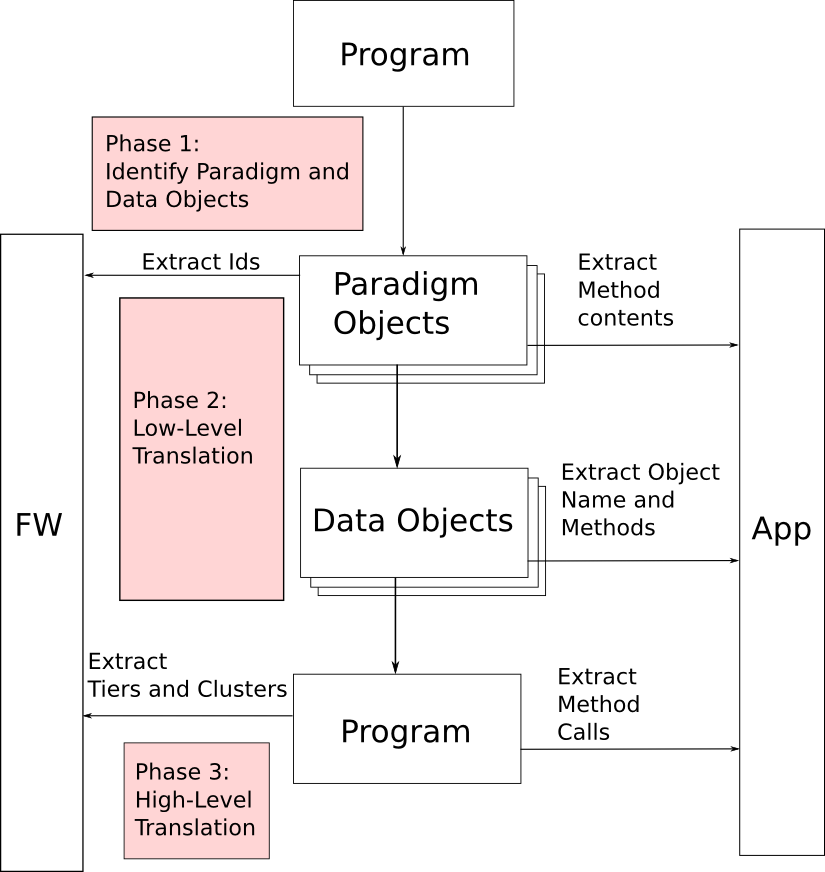
\includegraphics[scale=0.4]{translation.png}
\caption{Overview of the translation of SCJ programs to our model \label{tanslation}}
\end{center}
\end{figure}

\subsection{Phase One: Identify Objects}

When identifying the objects in an SCJ program it is useful to start at the top of the program hierarchy, at the Safelet, and work downwards, towards the schedulable objects. This methodology ensures that all the relevant objects in the program are captured.

Identifying the Safelet is relatively simple because there is only one in the program. Therefore to capture the Safelet we simply find the class that implements \texttt{javax.safetycritical.Safelet}. To capture the top-level mission sequencers, we identify any class that implements \texttt{javax.safetycritical.MissionSequencer} and could be returned by the Safelet's  \texttt{getSequencer()} method. 

To capture missions we begin by identifying any class that implements \texttt{javax.safetycritical.Mission} and may be returned by a top~level sequencer's \texttt{getNextMission()} method. Then we identify the schedulable objects that may be registered in the \texttt{initialize()} method of that mission. If this reveals any nested mission sequencers, then we identify any nested missions and their schedulable objects in the same way. This process is repeated until there are no more schedulable objects in the program that have not been identified. The location in the program hierarchy of each mission and schedulable is recorded to be used in phase three.

During this phase, if any objects are found that are not paradigm objects then they are classified as Data Objects. These will be translated, along with the Paradigm Objects, in phase two. Once all the objects in the program are identified, each paradigm object is assigned a unique identifier based on its class name.

\subsection{Phase Two: Low-Level Translation}

During this phase the objects identified in phase one are translated to \Circus{} processes using a set of rules. The rules are specific for each particular paradigm object and for any data object. The identifier for each paradigm object is give as a parameter to the relevant process in the framework model. The identifier, the contents of methods called by the framework model, and any program-specific methods of each paradigm object is used to construct its application process. For data objects, the name and methods of the object are used to construct an Oh\Circus{} class. 

\subsection{Phase Three: High-Level Translation}

The framework model of an SCJ program is organised in to several tiers, which each encapsulate several components. The basic structure of these tiers is the same for each program, but the framework model requires some program-specific information to ensure that the channels upon which the framework processes have to synchronise use the correct identifiers and do not cause the model to deadlock. The Safelet Tier contains the program's safelet and the top-level mission sequencers that were identified in phase one.

A Mission Tier contains several Clusters, each of which is a mission and its schedulable objects. Each program will have at least one mission tier (because a program must have at least one mission and one schedulable object) so our model always has Mission~Tier~0 to represent this. There may be as many other Mission~Tiers as needed to model the program. Each tier is composed of at least one cluster, which pairs a mission with its associated schedulable objects.

To capture Mission~Tier~ 0 we find each mission that may be returned by a top~level sequencer and each schedulable that may be registered in a Tier~0 mission's \texttt{initialize()} method. These processes are organised into clusters, where each mission is paired with its associated schedulables. 

The existence of other tiers is indicated by a Tier 0 cluster that contains a nested mission sequencer as one of its schedulable objects. To capture Mission~Tier~1, for example, we find any missions that may be returned by the \texttt{getNextMission()} method of a Tier~0 mission sequencer and their associated schedulables. Again, these mission and their associated schedulables are organised into clusters.  

One thing to note is that clusters controlled by the same mission sequencer will execute sequentially, whereas clusters controlled by different mission sequencers in the same tier will execute in parallel. 

\subsubsection{Example}

As an example of the way we identify the tiers within a program we consider the Aircraft mode change example. Figure~\ref{AircraftDiagram} shows the processes in our model of the program. 

\begin{figure}[!h]
\begin{center}
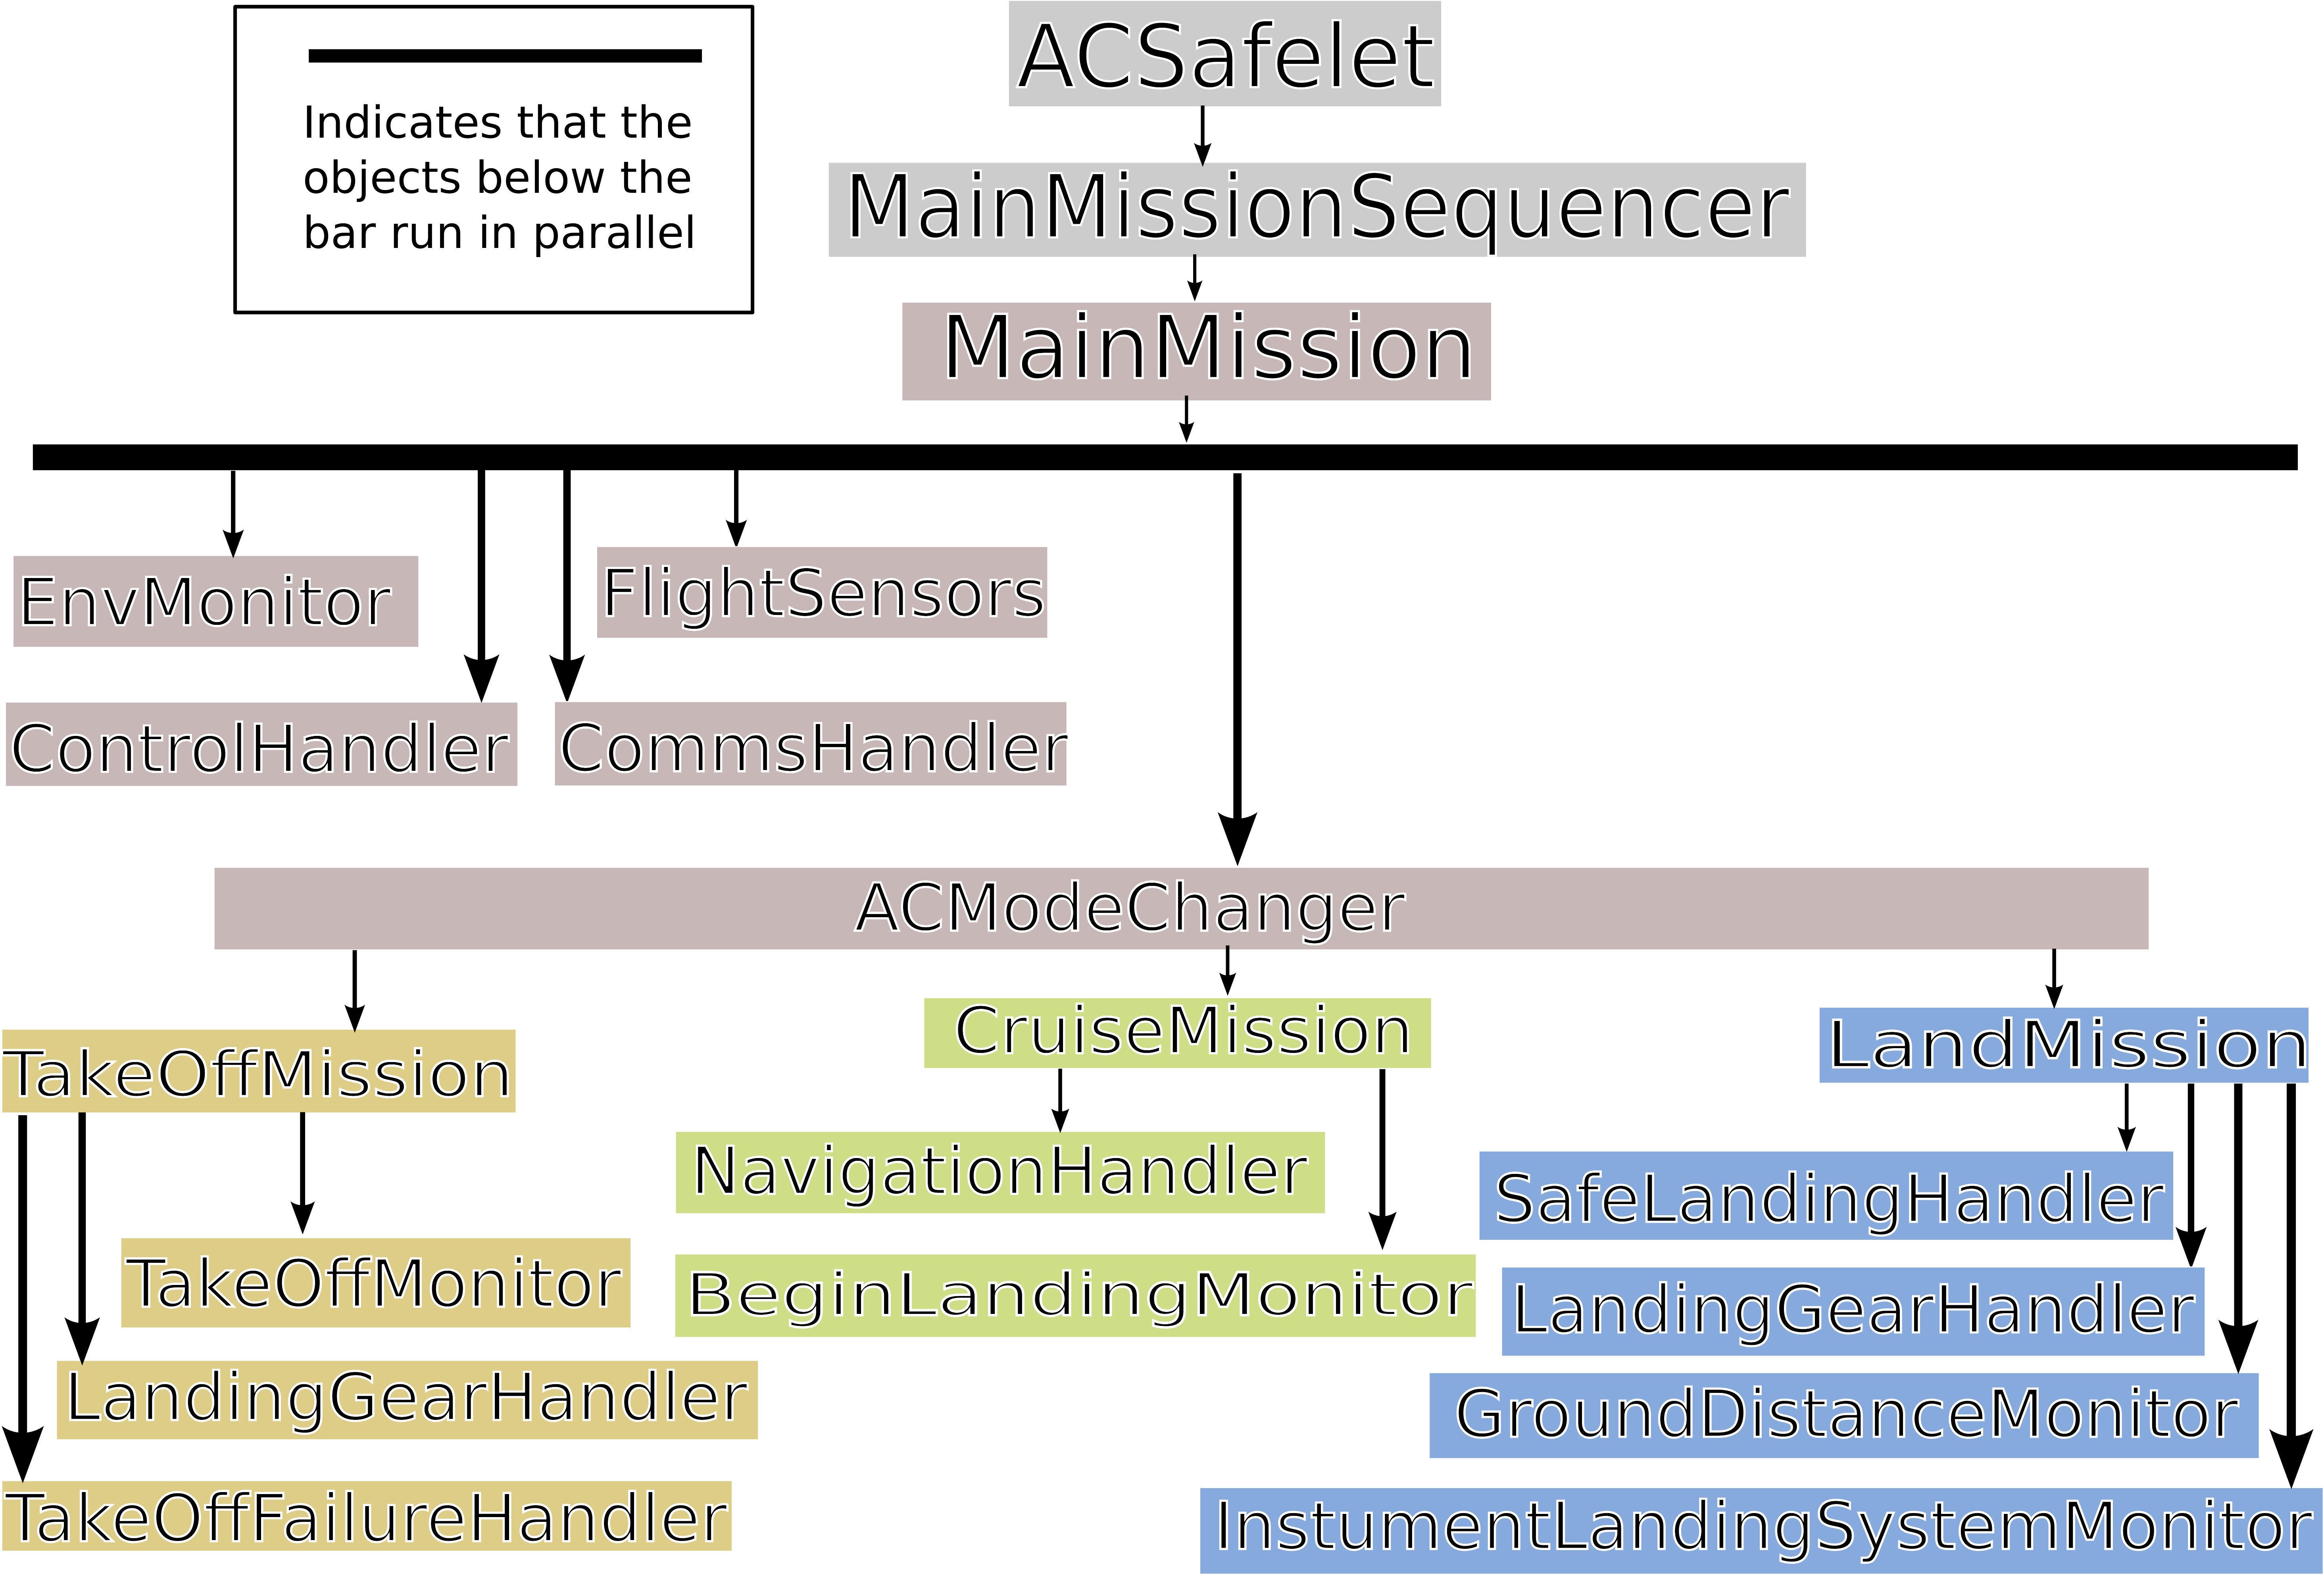
\includegraphics[scale=0.4]{AircraftStructure.png}
\caption{The processes in the model of the Aircraft mode change application \label{AircraftDiagram}}
\end{center}
\end{figure}

The Safelet~Tier contains the $ACSafelet$ and $MainMissionSequencer$ processes. Mission~Tier~0 contains one cluster that pairs the $MainMission$ process with the processes modelling the four handlers ($EnvMoniotr$, $FlightSensors$, $ControlHandler$, $CommsHandler$) and the $ACModeChanger$ process, which is the nested mission sequencer . 

Mission~Tier~1 contains three clusters. Each cluster pairs a single mission with the schedulable objects that it may register. One cluster pairs the $TakeOffMission$ process with the processes $TakfeOffMonitor$, $LandingGearHandler$, and $TakeOffFailureHandler$. The second cluster pairs the $CruiseMission$ process with the $NavigationHandler$ and $BeginLandingMonitor$ processes. The final cluster pairs the $LandMission$ process with the $SafeLandingHandler$, $LandingGearHandler$, $GroundDistanceMonitor$, and $InstrumentLandingSystemMonitor$ processes. 


\end{document}